\documentclass[a4paper,12pt]{article} % тип документа

% Поля страниц
\usepackage[left=2.5cm,right=2.5cm, top=2cm,bottom=2cm,bindingoffset=0cm]{geometry}
    
%Пакет дял таблиц   
\usepackage{multirow} 
    
%Отступ после заголовка    
\usepackage{indentfirst}


% Рисунки
\usepackage{subcaption,floatrow,graphicx,calc}
\usepackage{wrapfig}

% Создаёем новый разделитель
\DeclareFloatSeparators{mysep}{\hspace{1cm}}

% Ссылки?
\usepackage{hyperref}
\usepackage[rgb]{xcolor}
\hypersetup{				% Гиперссылки
    colorlinks=true,       	% false: ссылки в рамках
	urlcolor=blue          % на URL
}


%  Русский язык
\usepackage[T2A]{fontenc}			% кодировка
\usepackage[utf8]{inputenc}			% кодировка исходного текста
\usepackage[english,russian]{babel}	% локализация и переносы


% Математика
\usepackage{amsmath,amsfonts,amssymb,amsthm,mathtools, mathrsfs, wasysym}


\begin{document}
\begin{center}
	\footnotesize{ФЕДЕРАЛЬНОЕ ГОСУДАРСТВЕННОЕ АВТОНОМНОЕ ОБРАЗОВАТЕЛЬНОЕ 			УЧРЕЖДЕНИЕ ВЫСШЕГО ОБРАЗОВАНИЯ}\\
	\footnotesize{МОСКОВСКИЙ ФИЗИКО-ТЕХНИЧЕСКИЙ ИНСТИТУТ\\(НАЦИОНАЛЬНЫЙ 			ИССЛЕДОВАТЕЛЬСКИЙ УНИВЕРСИТЕТ)}\\
	\footnotesize{ФАКУЛЬТЕТ ОБЩЕЙ И ПРИКЛАДНОЙ ФИЗИКИ\\}
	\hfill \break
	\hfill\break
	\hfill\break
	\hfill \break
	\hfill \break
	\hfill \break
	\hfill \break
	\hfill \break
	\hfill \break
	\hfill \break
	\hfill \break
	\hfill \break
	\hfill \break
	\hfill \break
	\large{Лабораторная работа № 5.4.2 \\\textbf{Исследование энергетического спектра $\beta$-частиц и определение их максимальной энергии при помощи магнитного спектрометра.}}\\
	\hfill \break
	\hfill \break
	\hfill \break
	\begin{flushright}
		Серебренников Даниил\\
		Группа Б02-826м
	\end{flushright}
	\hfill \break
	\hfill \break
	\hfill \break
	\hfill \break
	\hfill \break
	\hfill \break
	\hfill \break
	\hfill \break
	\hfill \break
	\hfill \break
\end{center}
\begin{center}
	Долгопрудный, 2020 г.
\end{center}
\thispagestyle{empty}
\newpage
	\textbf{Цель работы:} с помощью магнитного спектрометра исследовать энергетический спектр $\beta$-частиц при распаде ядер $^{137}$Cs и определить их максимальную энергию.

\section{Теоретическая часть}
	
	Бета-распад - самопроизвольное превращение ядер, при котором их массовое число не изменяется, а заряд увеличивается или уменьшается на единицу.
	В данной работе:
	$$^A_Z X \to ^{\ \, A}_{Z+1} X + e^- + \widetilde{\nu} .$$
	
	Величина $W(p_e)$ является плотностью вероятности. Распределение электронов по энергии может быть вычислено теоретически. Для разрешенных переходов вероятность $\beta$-распада просто попрорциональна сатистическому весу.
	\begin{equation*}
		\label{eq:W}
		W(p_e)dp_e \propto p_e^2(E_m-E_e)^2 dp_e.
	\end{equation*}
	Кинетическая энергия электрона и его импульс связаны друг с другом обычной формулой:
	\begin{equation*}
		E = \sqrt{(p_ec)^2+(m_ec^2)^2}-m_ec^2
	\end{equation*}
	Выражение (\ref{eq:W}) приводит к спектру, имеющему вид широкого колокола. Кривая плавно отходит от нулся и стольже плавно, по параболе, касается оси абсцисс в области максимального импульса электронов.
	
	Дочерние ядра, возникающие в результате $\beta$-распада, нередко оказываются возбужденными. Возбужденные ядра отдают свою энергию либо излучая $\gamma$-квант, либо передвавая избыток энергии одному из электронов внутренних оболочек атома. Излучаемые в таком процессе электроны имеют строго определенную энергию и называются \textit{конверсионными}.
	
	Конверсия чаще всего происходит на оболочках K и L. Ширина конверсионной линии является чисто аппаратурной -- по ней можно оценить разрешающую силу спектрометра.
	
\newpage
\section{Экспериментальная установка}
	Блок-схема установки для изучения $\beta$-спектров изображена на рис. \ref{pic1}. Радиоактивный источник $^{137}$Cs помещен внутрь откачанной трубы. Электроны, сфокусированные магнитной линзой, попадают в счетчик. В газоразрядном счетчике они инициируют газовый разряд и тем самым приводят к появлению электрических импульсов на электродах, которые затем регистрируются пересчетным прибором.
	
	
	\thisfloatsetup{floatrowsep=mysep}	
	\begin{figure}[h!]
		\ffigbox{
			\begin{subfloatrow}[2]
				\ffigbox[\FBwidth]{\caption{}}%
				{\includegraphics[width=8cm,height=4cm]{shema.png}{\label{pic1}}}
				\ffigbox[\FBwidth]{\caption{}}%
				{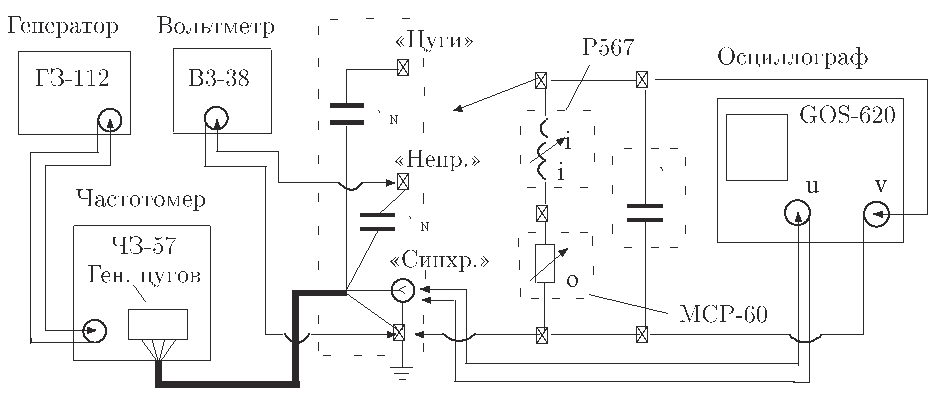
\includegraphics[width=8cm,height=4cm]{ustanovka.png}{\label{pic2}}}         
			\end{subfloatrow}
		}
		{\caption{Экспериментальная установка.}}
	\end{figure}

	Энергию $\beta$-частиц определяют с помощью $\beta$-спектрометров (рис.~\ref{pic2}). В работе используется магнитный спектрометр с <<короткой линзой>>. Отметим, что в течение всего опыта геометрия прибора остается неизменной, поэтому импульс сфокусированных электронов пропорционален величине тока:
	\begin{equation}
		\label{eq:pkI}
		\tag{$\star$}
		p_e = kI.
	\end{equation}

	Cвязь между числом частиц, регистрируемых установкой, и функцией $W(p_e)$ выражается формулой:
	\begin{equation*}
		N(p_e) \propto W(p_e)p_e,
	\end{equation*}
	откуда
	\begin{equation}
		\label{eq:fermi}
		\tag{$\star \star$}
		\frac{\sqrt{N}}{p_e^{3/2}} \propto E_m - E
	\end{equation}
	
	
	
	\newpage
	\section{Экспериментальные данные}
		
	
		\floatsetup[table]{capposition=top}	
		\begin{table}[H]
			\caption{Результаты измерений $\beta$-спектра.}
			\label{table:exp1}
			\begin{tabular}{|c|c|c|c|}
				\hline
				$I$, А & $\sigma_I$, A & $N$, с$^{-1}$ & $\sigma_N$, с$^{-1}$ \\ \hline
				0,00   & 0,02          & 1,34          & 0,05                 \\ \hline
				0,50   & 0,02          & 1,42          & 0,05                 \\ \hline
				1,00   & 0,02          & 2,9           & 0,1                  \\ \hline
				1,51   & 0,02          & 4,7           & 0,2                  \\ \hline
				1,55   & 0,02          & 5,8           & 0,2                  \\ \hline
				1,60   & 0,02          & 7,0           & 0,3                  \\ \hline
				1,70   & 0,02          & 7,8           & 0,3                  \\ \hline
				1,90   & 0,02          & 8,1           & 0,3                  \\ \hline
				2,00   & 0,02          & 8,0           & 0,3                  \\ \hline
				2,15   & 0,02          & 7,6           & 0,3                  \\ \hline
				2,25   & 0,02          & 7,2           & 0,3                  \\ \hline
				2,40   & 0,02          & 6,4           & 0,2                  \\ \hline
				2,50   & 0,02          & 5,2           & 0,2                  \\ \hline
				2,60   & 0,02          & 4,4           & 0,2                  \\ \hline
				2,75   & 0,02          & 3,5           & 0,1                  \\ \hline
				2,90   & 0,02          & 3,3           & 0,1                  \\ \hline
				3,00   & 0,02          & 3,8           & 0,1                  \\ \hline
				3,10   & 0,02          & 7,3           & 0,3                  \\ \hline
				3,15   & 0,02          & 9,6           & 0,4                  \\ \hline
				3,20   & 0,02          & 10,2          & 0,4                  \\ \hline
				3,25   & 0,02          & 10,5          & 0,4                  \\ \hline
				3,30   & 0,02          & 9,4           & 0,3                  \\ \hline
				3,40   & 0,02          & 7,2           & 0,3                  \\ \hline
				3,50   & 0,02          & 3,8           & 0,1                  \\ \hline
				3,60   & 0,02          & 2,37          & 0,09                 \\ \hline
				3,70   & 0,02          & 1,57          & 0,06                 \\ \hline
				3,80   & 0,02          & 0,87          & 0,03                 \\ \hline
				3,90   & 0,02          & 0,60          & 0,02                 \\ \hline
				4,00   & 0,02          & 0,75          & 0,03                 \\ \hline
				4,10   & 0,02              & 0,56          & 0,02                 \\ \hline
			\end{tabular}
		\end{table}
		
		
	
		\floatsetup[table]{capposition=top}	
		\begin{table}[H]
			\caption{Результаты измерения фона.}
			\label{table:exp2}
			\begin{tabular}{|c|c|c|c|}
				\hline
				$I$, A & t, с & $N_\text{ф}$, c$^{-1}$ & $\sigma_{N_\text{ф}}$, c$^{-1}$ \\ \hline
				0,00   & 100  & 1,3                    & 0,1                             \\ \hline
				4,10   & 100  & 0,54                   & 0,07                            \\ \hline
			\end{tabular}
		\end{table}
	
	\newpage
	\section{Обработка результатов}
		По результатам измерений (табл.~\ref{table:exp1}) построим график cпектра $\beta$-распада атома $^{137}$Cs и откалибруем его. Для этого пересчитаем значения силы тока в импульс по формуле (\ref{eq:pkI}). Коэффициент $k$ определим по известной конверсионной линии:
			$$1013,5 \ \text{кэВ} = kcI_0,$$
		где $c$ -- скорость света, $I_0 = 3,25$ А -- сила тока, при которой наблюдается конверсионный пик. Получаем, что $$k = (312 \pm 2) \frac{\text{кэВ}}{c\cdot\text{А}}.$$
		
		Сдвиг графика по оси ординат сделаем на величину радиационного фона $N_\text{ф}$ при $I = 4,10$ А (табл.~\ref{table:exp2}), так как в этом случае график касается оси абсцисс в области максимальной энергии, что соответствует теоретической зависимости.
		\begin{figure}[h!]
			\begin{floatrow}
				\ffigbox[\FBwidth]{\caption{Спектр $\beta$-распада атома $^{137}$Cs.}\label{fig:spectre1}}%
				{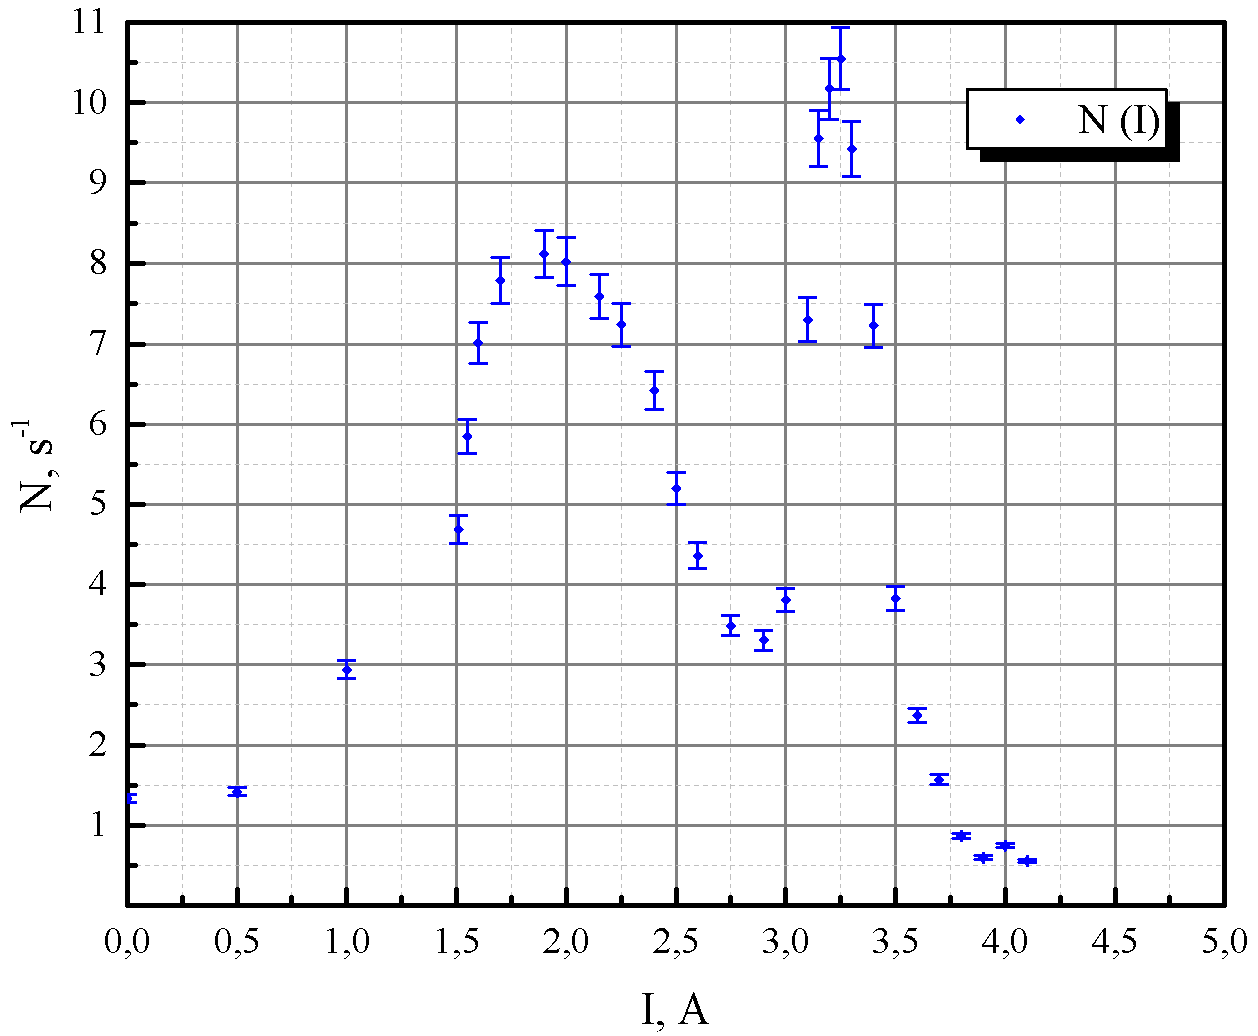
\includegraphics[width=8cm,height=7cm]{graph0.pdf}}
				\ffigbox[\FBwidth]{\caption{Откалиброванный график.}\label{fig:spectre2}}%
				{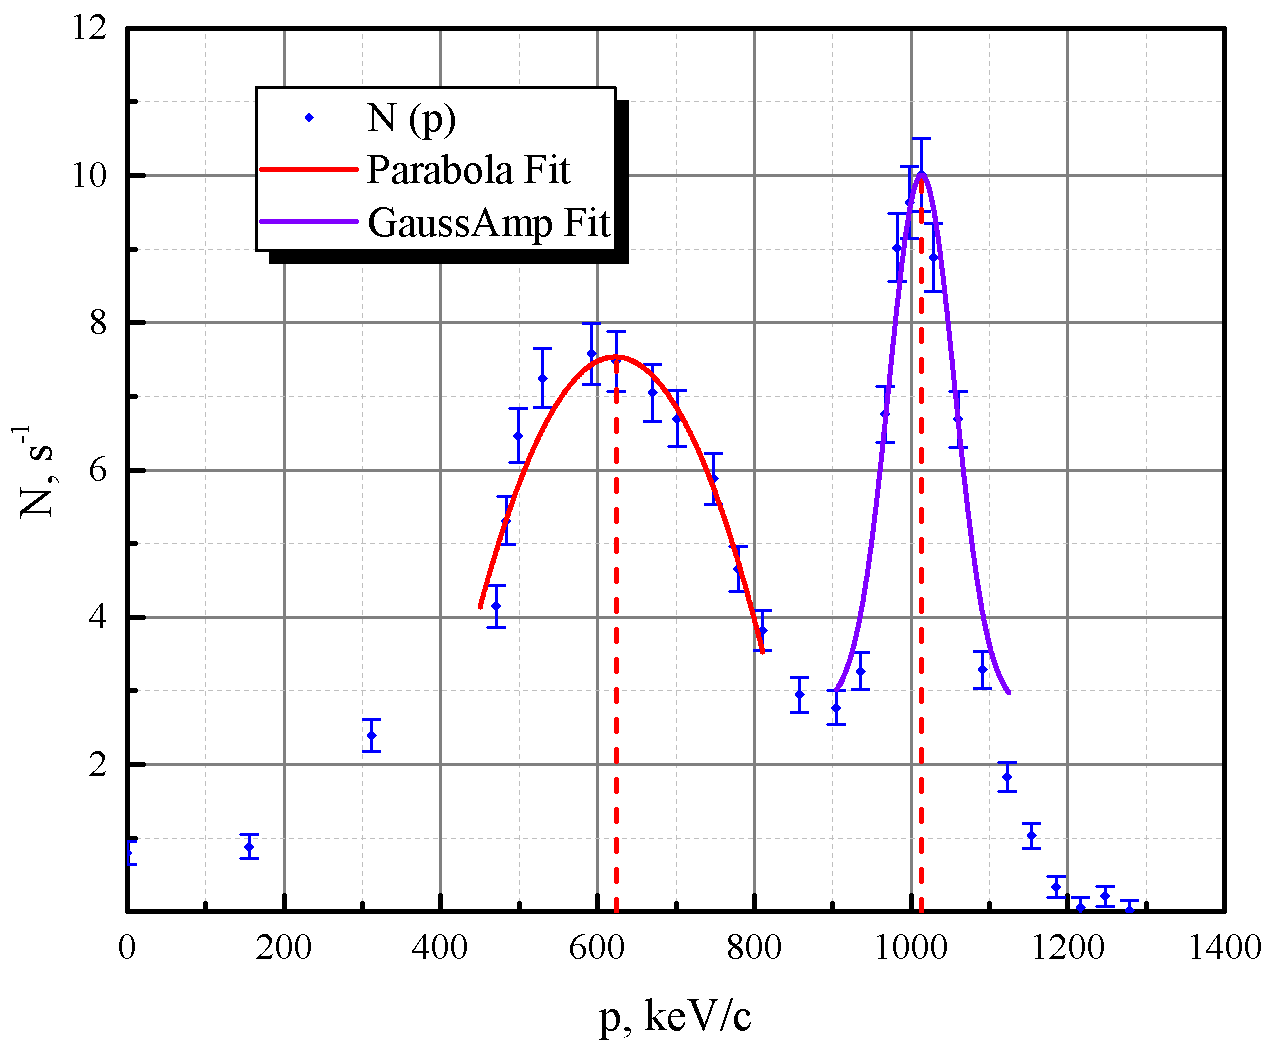
\includegraphics[width=8cm,height=7cm]{graph1.pdf}}     
			\end{floatrow}
		\end{figure}
		
		\newpage
		Определим максимальную энергию $\beta$-спектра. Анализ рис.~\ref{fig:spectre2} в таком случае даст достаточно грубый результат, так как нам придётся ограничииться исследованием точек у самой верхней границы спектра. Эти точки измерены с наименьшей статистической точностью. Однако мы можем уменьшить ошибку определения максимальной энергии посредством процедуры Ферми-Кюри. Для этого мы отложим по оси ординат величину $\sqrt{N}/p^{3/2}$, а по оси абсцисс энергию $\beta$-частиц (с учётом того, что энергия электронов внутренней конверсии $^{137}$Cs равна 634, кэВ). В таком случае мы задействуем большинство экспериментальных точек, и прежде всего точки середины $\beta$-спектра, которые измерены с наилучшей точностью.
		
		\begin{figure}[h!]
			\begin{floatrow}
				\ffigbox[\FBwidth]{\caption{График Ферми-Кюри.}\label{fig:fermi-kuri}}%
				{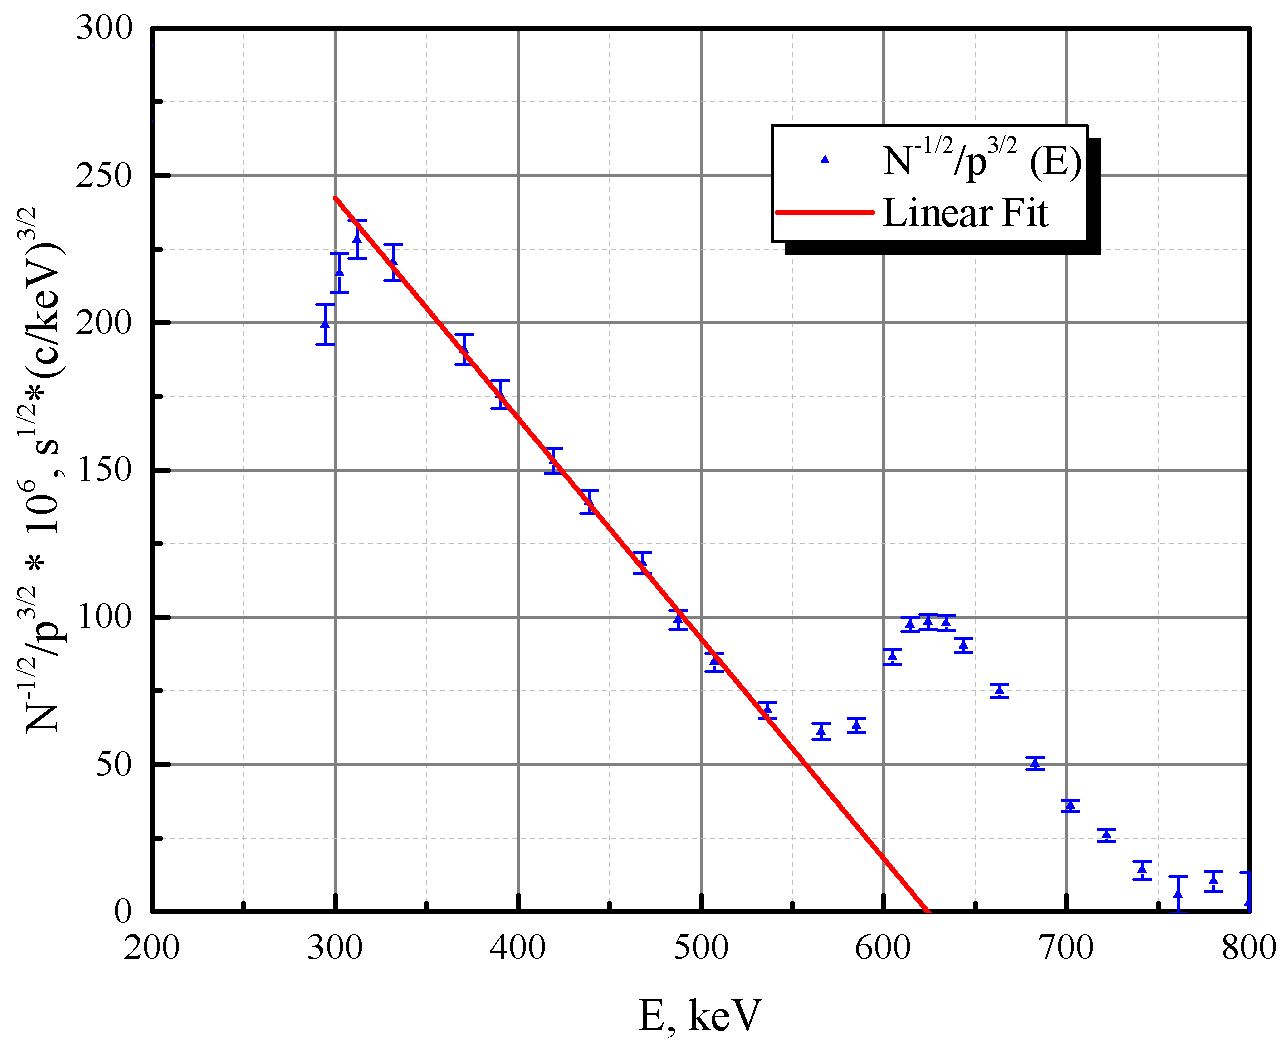
\includegraphics[width=8cm,height=7cm]{graph2.pdf}}   
			\end{floatrow}
		\end{figure}
	
		\floatsetup[table]{capposition=top}	
		\begin{table}[H]
			\caption{Результаты линейной аппроксимации.}
			\label{table:Emax}
			\begin{tabular}{|c|c|c|}
				\hline
				& $a$, $\text{с}^{1/2} \cdot {c^{3/2}} \cdot\text{кэВ}^{-5/2}$ & $b$, $\text{с}^{1/2} \cdot {c^{3/2}} \cdot\text{кэВ}^{-3/2}$ \\ \hline
							Величина    & -0,748                                                        & 467                                                                     \\ \hline
							Погрешность & 0,018                                                         & 9                                                                       \\ \hline
						\end{tabular}
		\end{table}
		Ясно, что $E_m = - \frac{b}{a}$ и $\sigma_{E_m} = E_m \sqrt{\left(\frac{\sigma_a}{a}\right)^2 + \left(\frac{\sigma_b}{b}\right)}$, откуда $E_m =(620 \pm 20) \ \text{кэВ}.$
		

\newpage
\section{Обсуждение результатов и выводы}
	В ходе лабораторной работы с помощью магнитного спектрометра мы исследовали энергетический спектр $\beta$-частиц при распаде ядер $^{137}$Cs. Калибровку спектрометра осуществили по энергии электронов внутренней конверсии.
	
	Анализ графика (рис.~\ref{fig:spectre2}) показывает, что точки купола достаточно хорошо приближаются параболой. Такой вид зависимости согласуется с теоретической. Конверсионный же пик оказывается можно приблизить Гауссовым распределением. Заметим, что в окрестности нуля спектр положителен -- эти точки требуют повторного измерения.
	
	Также мы определили максимальную энергию $E_m = 620$ кэВ вылетающих электронов при $\beta$-распаде ядря $^{137}$Cs методом Ферми-Кюри  с ошибкой в 3\%.


\end{document}